\documentclass[12pt]{article}
\usepackage{graphicx}
\usepackage{subcaption}
\setlength{\parindent}{0pt}
\setlength{\parskip}{10pt} % block paragraphs
\usepackage{bm}
\begin{document}

\title*{\centerline{\huge{CAP 5619 \-- Deep and Reinforcement Learning}}}
\author*{\centerline{Homework 2 Hua Huang}}%unnumbered centered head

\section{Problem 1}
For re\--LU, inactive learning region for $z<0$, fast learning region
for $ z>0$, undefined for $z=0$;\\
For sigmoid, active learning region for $-2.063\leq z \leq 2.063$,
slow learning region for $z \leq -2.063$ and $2.063\leq z$;\\
For piece\--wise linear function, fast learning region for 
$-1< z < 1$, slow learning region for $z<-1$ and $z>1$, undefined for
$z=\pm 1$;\\
For Swish linear function, slow learning region for $z<-0.1825$,
active learning region for $-0.1825 \leq z \leq 0.1825$, fast learning
region for $z>0.1825$.
\begin{figure}[h]
    \centering
    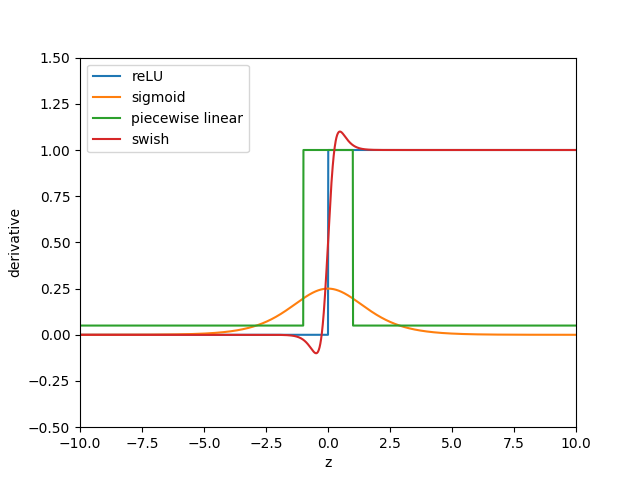
\includegraphics [scale=0.5]{prob1.png}
    \caption {Derivative for activation functions}
\end{figure}

\section{Problem 2}
(1) For Alg 6.1, it's a forward propogation:\\
Line $1\sim 3$, set the units of 1st layer to be the input values;\\
Line 4: Since it has already been assumed nodes of the graph have been
ordered in such a way that we can compute their output one after the
other, starting at $u^{(n_i+1)}$ and going up to $u^n$, we can compute
the forward propogation from $n_i+1$ to $n$ incrementally.\\
Line 5: collect the sets of argument $A^{(i)}$ which compromises the
values of parents of $u^{(i)}$.\\
Line 6: Apply the operation (for example, dot product, and then
activation function) to $A^{(i)}$.\\
Line 8: Return output scalar $u^n$.\\\\
For Alg 6.2, it's the back-propogation:\\
Line $1\sim2$: run forward propogation first;\\
Line $3\sim5$: initialize the grad table;\\
Line 6: Set grad table $[u^{(n)}]$ to be 1, since $\frac{du^{(n)}}{du^{(n)}}=1$;\\
Line 7: Since it has already been assumed nodes of the graph have been
ordered in such a way that we can compute their output one after the
other, starting at $u^{(n_i+1)}$ and going up to $u^n$, we can compute
the backward propogation from $n-1$ to $n_i+1$ to $1$ decrementally.\\
Line $8\sim9$: For current layer, calculate the grad table by
multiplying the stored grad values in children units with the
derivative of the children unit with respect to parent node, and sum
over all the products.\\
Line 11: Return the grad table for units $u^{(i)}, i\in{1, ...,
n_i}$.\\\\
(2) They are the same order of number of computations because all the
backpropogation uses the stored values, namely all the intermidiate
grad are just calculated once. Actually the grad is calulated whenever
there is a edge connection in the graph, and it's calculated only
once. In forward computation, similarly the dot product between the
weigths of each layer and the units in corresponding layer is also
computed once, the the compuation is done once for each and every edge
in the graph. In summary, the edges are the same for forward and
backward computation, so the two algorithms require the same order of
the number of computations.

\section{Problem 3}
4 hidden layers (Multiple perceptron layer, MLP) are used here, each layer has $32$ 
units, in total, there are 128 hidden units.
\begin{figure}[h]
    \centering
    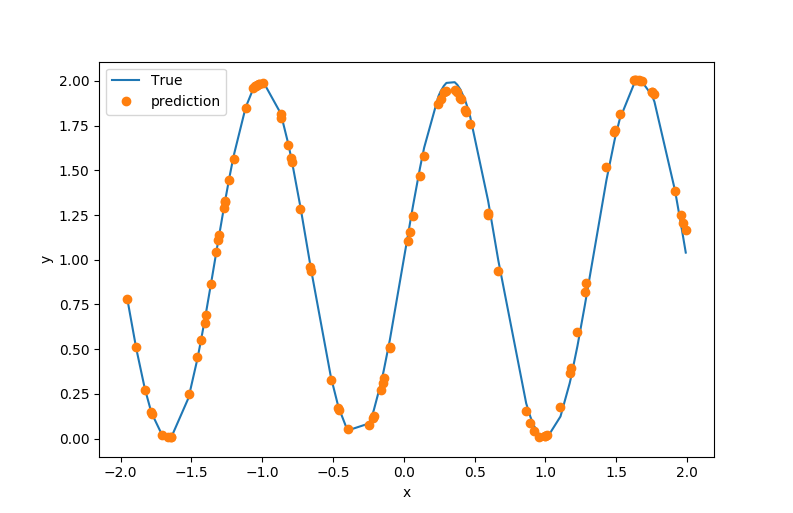
\includegraphics [scale=0.5]{Figure_3.png}
    \caption {MLP approximation results}
\end{figure}

\section{Problem 4}
(1) There are 100 hidden units in the hidden layer, and 20 output
units. The input dimension (also input units) is 100, There are $20\times(100+1)=2020$ connections.\\
(2) the largest $z_i$ is for $i=3$, namely the 4th class.\\
(3) Since we have 
\begin{eqnarray}
    \frac{dJ}{dz_i}=q_i-p_i \\
    \frac{dJ}{d\bm{w}}=\frac{dJ}{d\bm z}\frac{d\bm z}{d\bm w}=(\bm{q-p})\bm{h}^T\\
    \frac{dJ}{d\bm{b}}=\frac{dJ}{d\bm z}\frac{d\bm z}{d\bm b}=\bm{q-p}
\end{eqnarray}
in which $\bm q$ is the softmax output, and $\bm p$ is the true classes. So in
total, there will be 97 positive $d\bm W$ which are larger then
$\frac{0.001}{0.1}$, and will decrease, and 10 negative $d\bm W$ which
smaller then $-\frac{0.001}{0.1}$, and will increase, the remainning
1893 $d\bm W$ will basically remain the same. \\
For bias, there will be 14 decreased biases, 1 increased, and 5
unchanged.
\end{document}


